\documentclass[a4]{article}
\usepackage{geometry}
\geometry{verbose,tmargin=2.5cm,bmargin=2.5cm,lmargin=3cm,rmargin=3cm}
\usepackage{amsmath,amssymb,amsthm}
\usepackage{graphicx}
\graphicspath{{graphics/}}
\usepackage[utf8]{inputenc}
\usepackage{fancyvrb}
\usepackage{hyperref}
\usepackage{lscape}
\usepackage{adjustbox}
\usepackage{verbatim}

\title{MultiFEBE \\ Tutorial 4: static analysis of an elastic straight cantilever beam with finite elements}
\author{\'A.G. Vega-Artiles}
\date{September 2022}

\begin{document}

\maketitle

\tableofcontents 

\section{Problem description}

In this fourth tutorial, a static analysis of an elastic straight cantilever beam is performed using the Finite Element Method (FEM), i.e. finite elements. Figure \ref{fig:beam} shows the geometry. Required material and geometric properties are the Young's modulus $E$, the Poisson's ratio $\nu$, the length $L$ and the square-shaped cross section $1 \medspace \mathrm{m} \medspace \mathrm{x} \medspace 1 \medspace \mathrm{m}$. Self-weight is not considered. 

The analytical solution to this problem can be obtained by means of the following equations:

\begin{equation}
	\begin{array}{l}
		I = \frac{ab^3}{12} \\
		u_z = \frac{FL^3}{3EI} \\
		\theta = \frac{FL^2}{2EI}
	\end{array}
\end{equation}

The problem is solved for $L=10$ $\mathrm{m}$, $E=200\cdot 10^9$ $\mathrm{N/m^2}$, $\nu=0.26$, $F=1000$ $\mathrm{N}$ and the results are the following: 

\begin{equation}
	\begin{array}{l}
		E = 200\cdot 10^9 \medspace \mathrm{N/m^2} \\
		I = 1/12 \medspace \mathrm{m^4} \\
		u_z = 2\cdot 10^{-5} \medspace \mathrm{m}\\
		\theta =  -3\cdot 10^{-6} \medspace \mathrm{rad}\\
		N_{x} = 0\\
		V_{z} = 1000 \medspace \mathrm{N}\\
		M_{y} = -1000\cdot(10-x)\medspace \mathrm{N}
	\end{array}
\end{equation}

\begin{figure}[h]
	\centering
	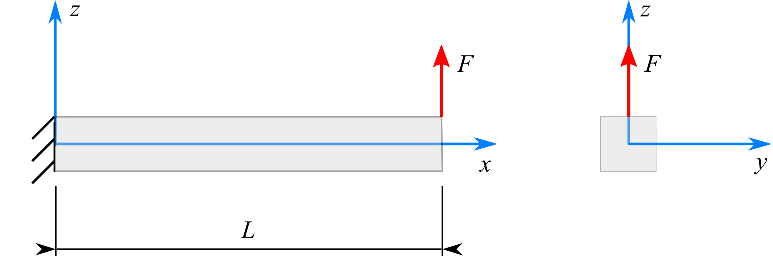
\includegraphics{beam.eps}
	\caption{Problem layout.}
	\label{fig:beam}
\end{figure}

\section{Pre-processing} 
Pre-processing in MultiFEBE consists of defining the geometry and mesh of the problem. There are three ways to do such definition: directly from the input file (mode = 0), from another file in the native format (mode = 1) or from another file in the Gmsh MSH file format version 2.2 (mode = 2). 

In the current example the problem definition will be read from the input file. 

\subsection{Input data file}
Solving in MultiFEBE consists of running the software by specifying several options in the following sections\footnote{See reference manual.}: [problem], [settings], [materials], [regions], [conditions over nodes], etc.

The first part to configurate is the problem definition in the section [problem]. This example is a 3D static mechanical problem.

\begin{Verbatim}	
[problem]
type = mechanics
analysis = static
n = 3D
\end{Verbatim}

As the problem has just one material, the section [materials] will need two lines: a first line for the number of materials in the model and a second line for the properties such as tag, type, E and $\nu$.

\begin{Verbatim}
[materials]
1
1 elastic_solid E 200.E9 nu 0.26
\end{Verbatim}

Next step is to configurate the mesh. Mesh definition requires three sections: [parts], [nodes] and [elements]. 

In the section [parts], groups with a similar significance are defined. The first line specifies the number of parts (1) and a line per part by indicating the part identifier (1) and the part name (beam).    

The nodes are defined in the section [nodes]. The first line specifies the number of nodes (5) and a line per node by indicating the node identifier and its coordinates (x y z).    

In the section [elements], all the elements of the model are defined. The first line indicates the number of elements (4) and a line per element indicating the element identifier, the type of element (line2 = line element with 2 nodes), the number of auxiliary tags (1), the part identifier (1) and a list of identifiers corresponding to the nodes of the element.

\begin{Verbatim}	
[parts]
1
1 beam
\end{Verbatim}

\begin{Verbatim}	
[nodes]
5
1 0. 0. 0.
3 2.5 0. 0.
4 5.0 0. 0.
5 7.5 0. 0.
2 10. 0. 0.
\end{Verbatim}

\begin{Verbatim}	
[elements]
4
1 line2 1 1 1 3
2 line2 1 1 3 4
3 line2 1 1 4 5
4 line2 1 1 5 2
\end{Verbatim}

The section [fe subregions] indicates the number of fe subregions in the first line (1) and a line per subregion indicating the subregion identifier (1) and the part identifier (1). The last two zeros at the end of the line are mandatory and they are going to be used in the
future for additional features.

\begin{Verbatim}
[fe subregions]
1
1 1 0 0
\end{Verbatim}

In the section [cross sections], it is necessary to specify the number of cross sections in the first line and a line per cross section by indicating the type of fe (strbeam\_eb = straight beam, Euler–Bernoulli model), number of fe subregions related to the cross section (1), fe subregion identifier (1), type of cross section (rectangle), y dimension (1), z dimension (1), reference vector for y' direction (0. 1. 0.).

\begin{Verbatim}
[cross sections]
1
strbeam_eb 1 1 rectangle 1. 1. 0. 1. 0.
\end{Verbatim}

The format of the section [regions] consists of a first line indicating the number of regions (1). Furthermore, for each region there must be a block of data consisting of several lines of data. The first one is the region identifier and the region class (discretization method) (1 fe). As the region is a FE region, then the second line indicates the number of subregions (1) and their identifiers (1). The third line defines the material (material 1). 

\begin{Verbatim}	
[regions]
1
1 fe
1 1
material 1
\end{Verbatim}

In the section [conditions over nodes], all boundary conditions over nodes will be specified. As a 3D model, there are 6 lines for every boundary condition. Every line has two digits, where the first one indicates the type of condition (0 for displacement and 1 for force) and the second one the value. In case of displacement, firstly the displacements $u_x, u_y, u_z$ and then the rotations $\theta_x, \theta_y, \theta_z$. In case of force, firstly the forces $F_x, F_y, F_z$ and then the moments $M_x, M_y, M_z$. 

\begin{Verbatim}	
[conditions over nodes]
node 1: 0 0
        0 0
        0 0
        0 0
        0 0
        0 0

node 2: 1 0
        1 0
        1 1000
        1 0
        1 0
        1 0
\end{Verbatim}

The whole data file applied to the problem is the following:

\begin{Verbatim}
[problem]
type = mechanics
analysis = static
n = 3D

[materials]
1
1 elastic_solid E 200.E9 nu 0.26

[parts]
1
1 beam

[nodes]
5
1 0. 0. 0.
3 2.5 0. 0.
4 5.0 0. 0.
5 7.5 0. 0.
2 10. 0. 0.

[elements]
4
1 line2 1 1 1 3
2 line2 1 1 3 4
3 line2 1 1 4 5
4 line2 1 1 5 2

[fe subregions]
1
1 1 0 0

[cross sections]
1
strbeam_eb 1 1 rectangle 1. 1. 0. 1. 0.

[regions]
1
1 fe
1 1
material 1

[conditions over nodes]
node 1: 0 0
        0 0
        0 0
        0 0
        0 0
        0 0

node 2: 1 0
        1 0
        1 1000
        1 0
        1 0
        1 0
\end{Verbatim}

\section{Results and discussion}

The results for the current example are in Table \ref{tab:beam_results}.

\begin{table}[h!]
	\begin{center}
		\begin{tabular}{|*{4}{c}|}
			\hline
			Node & Variable & Analytical solution & Numerical solution \\
			\hline
			1 & $u_z$ & 0 & 0.00\\
			\hline
			2 & $u_z$ & $ 20\cdot 10^{-6} $ & $ 20.00\cdot 10^{-6} $\\
			\hline
			1 & $\theta$ & 0 & $0.00$ \\
			\hline
			2 & $\theta$ & $ -3\cdot 10^{-6} $ & $-3.00\cdot 10^{-6}$ \\
			\hline
			1 & $N_{x}$ & 0 & 0.00 \\
			\hline
			2 & $N_{x}$ & 0 & 0.00 \\
			\hline
			1 & $V_{y}$ & $ 1\cdot 10^{3} $ & $ 1.00\cdot 10^{3} $ \\
			\hline
			2 & $V_{y}$ &$ 1\cdot 10^{3} $ & $ 1.00\cdot 10^{3} $ \\
			\hline
			1 & $M_{y}$ & $ -10\cdot 10^{3} $ & $-10.00\cdot 10^{3}$ \\
			\hline
			2 & $M_{y}$ & 0 & $-47.18\cdot 10^{-12}$ \\
			\hline
		\end{tabular}
	\end{center}
	\caption{Results.}
	\label{tab:beam_results}
\end{table}

It can be seen that the numerical solution is in perfect agreement with the analytical solution.

\end{document}
